% 编译：xelatex scheduler_report.tex（两遍）
\documentclass[UTF8,a4paper,10pt,fontset=fandol]{ctexart}
\usepackage[margin=2cm]{geometry}
\usepackage{graphicx,booktabs,hyperref,xcolor,listings}
\hypersetup{colorlinks=true,linkcolor=blue!50!black}
\setlength{\emergencystretch}{3em}
\lstset{language=C,basicstyle=\ttfamily\footnotesize,breaklines=true,columns=fullflexible,keepspaces=true,frame=single,rulecolor=\color{black!20},aboveskip=0.5em,belowskip=0.5em}
\newcommand{\code}[1]{\texttt{\detokenize{#1}}}
\begin{document}
\begin{center}
{\Large\bfseries 进程优先级调度实验报告}\\[0.5em]
姓名：赵心瑞\qquad 学号：24307140096
\end{center}

\section{核心修改与说明}
实验在单 CPU 下实现两级优先级调度：1 为低优先级，2 为高优先级；优先选择最高优先级的可运行进程，同优先级采用轮转。

\textbf{进程属性与系统调用。}在 \code{kernel/proc.h} 的 \code{struct proc} 中新增受进程锁保护的 \code{int priority;}，在 \code{allocproc()} 成功返回前执行 \code{p->priority = 1;}，保证新进程及复用槽位均使用默认值，不在 \code{fork()} 中继承父进程优先级。新增处理函数如下：
\begin{lstlisting}
uint64
sys_setpri(void) {
  int pri;
  argint(0, &pri);

  if (pri != 2 && pri != 1) {
    return -1;
  }

  struct proc* p = myproc();
  acquire(&p->lock);
  p->priority = pri;
  release(&p->lock);
  return 0;
}
\end{lstlisting}
用户接口为 \code{int setpri(int);}。在 \code{user/usys.pl} 添加入口，在 \code{kernel/syscall.h} 分配编号 22，并在 \code{kernel/syscall.c} 声明处理函数、注册分发表。参数通过 \code{argint(0, &pri)} 获取；非法值返回 $-1$ 且不修改原值，合法值在进程锁保护下写入并返回 0。

\textbf{调度策略。}调度器每轮先扫描所有 \code{RUNNABLE} 进程，得到最高优先级；再从持久保存的 \code{next} 位置循环查找匹配进程。每运行一个进程便返回外层循环，重新判断最高优先级；起点移至所选进程的下一槽位，避免靠前进程长期占用同级调度机会。核心实现见下一页。

所有状态及优先级检查均持有对应的 \code{p->lock}，保留原有上下文切换、锁交接及空闲等待逻辑。\code{SLEEPING} 进程不参与优先级比较，因此高优先级进程睡眠时低优先级进程仍可运行。每轮两次扫描的时间复杂度为 $O(\mathrm{NPROC})$；严格优先级可能使低优先级进程饥饿，本实验未加入老化机制。

\clearpage
\subsection*{scheduler() 核心代码（省略原注释）}
\begin{lstlisting}
void
scheduler(void)
{
  struct proc *p;
  struct cpu *c = mycpu();
  c->proc = 0;
  int next = 0;
  for(;;){
    intr_on();
    int highest = 0;
    for (p = proc; p < &proc[NPROC]; p++) {
      acquire(&p->lock);
      if (p->state == RUNNABLE && p->priority > highest) {
        highest = p->priority;
      }
      release(&p->lock);
    }
    int found = 0;
    for(int i = 0; i < NPROC; i++) {
      int index = (next + i) % NPROC;
      p = &proc[index];
      acquire(&p->lock);
      if(p->state == RUNNABLE && p->priority == highest) {
        p->state = RUNNING;
        c->proc = p;
        swtch(&c->context, &p->context);
        c->proc = 0;
        found = 1;
        next = (index + 1) % NPROC;
      }
      release(&p->lock);
      if (found) {
        break;
      }
    }
    if(found == 0) {
      intr_on();
      asm volatile("wfi");
    }
  }
}
\end{lstlisting}

\clearpage
\section{结果与分析}
使用 \code{make CPUS=1 SCHEDTEST=1 qemu} 启动，分别测试原调度器与优先级调度器；两者均保留相同的 \code{setpri} 接口和测试负载。\code{setpritest} 对 2、1、0、3、$-1$ 的返回值检查全部通过。

下表按截图记录 \code{start/finish}，单位为从统一释放时刻起计算的 tick：
\begin{center}
\begin{tabular}{llcc}
\toprule
测试 & 进程优先级 & 修改前 start/finish & 修改后 start/finish\\
\midrule
\code{schedtest 1 1} & 1（pid 5） & 0/2 & 0/2\\
                      & 1（pid 6） & 1/3 & 1/3\\
\code{schedtest 1 2} & 1（pid 8） & 0/3 & 1/3\\
                      & 2（pid 9） & 1/3 & 0/1\\
\bottomrule
\end{tabular}
\end{center}
同优先级测试前后结果一致，与轮转执行一致。不同优先级时，原调度器先执行低优先级进程，两个进程均在 tick 3 完成；修改后，高优先级进程在 tick 0 开始、tick 1 完成，低优先级进程在 tick 1 开始，体现了优先级选择效果。总完成时刻仍为 tick 3，说明本实验主要改变执行顺序与高优先级响应，而非提高计算吞吐量。

\code{start/finish} 为墙钟时间，包含调度等待，并非进程实际占用 CPU 的时间；tick 粒度较粗，单次结果受时序影响。上述分析以本次截图为准。

\begin{figure}[htbp]
\centering
\begin{minipage}[t]{0.49\textwidth}
\centering\textbf{修改前}\\[0.5em]
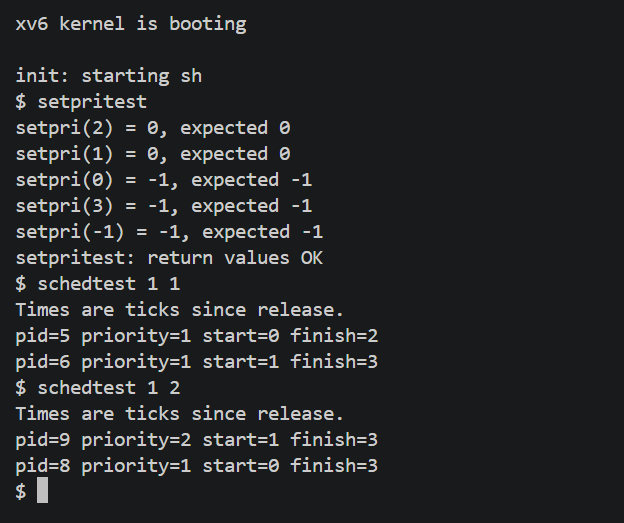
\includegraphics[width=\linewidth]{result-1.png}
\end{minipage}\hfill
\begin{minipage}[t]{0.49\textwidth}
\centering\textbf{修改后}\\[0.5em]
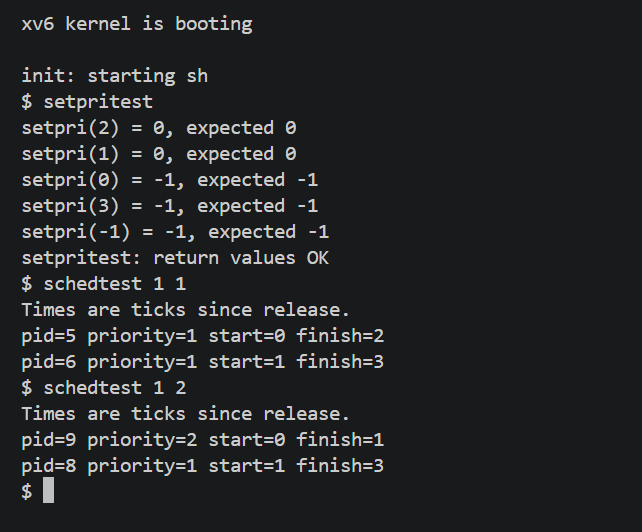
\includegraphics[width=\linewidth]{result-2.png}
\end{minipage}
\caption{系统调用返回值检查与调度结果对比。}
\end{figure}
\end{document}
